\subsection{Bestimmung der Schwingdauer}
Für die Messung der Schwingdauer wird die Apparatur wie in Abbildung \ref{mess1}
verwendet.
\begin{figure}[H]
  \centering
  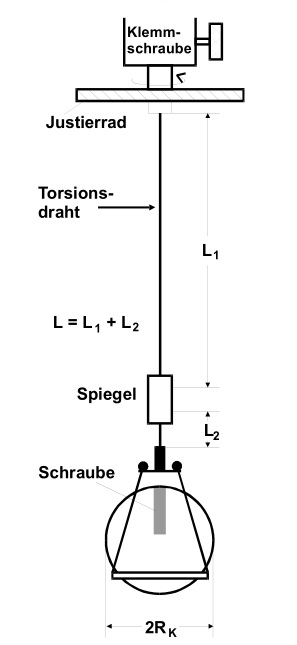
\includegraphics[height=0.5\textwidth]{bilder/aufbau.jpg}
  \caption{Skizze der Messapparatur\cite{102}}
  \label{mess1}
\end{figure}
Über den angebrachten Spiegel wird ein gebündelter Lichtstrahl, wie in
Abbildung \ref{periode} reflektiert.
\begin{figure}[H]
  \centering
  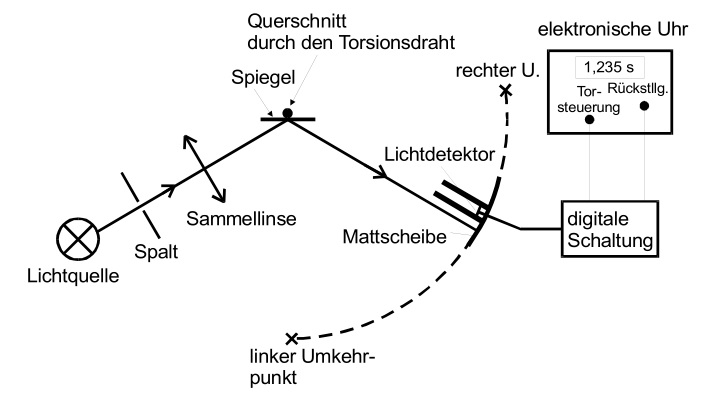
\includegraphics[width=0.8\textwidth]{bilder/periode.jpg}
  \caption{Schematische Darstellung der Periodendauermessung\cite{102}}
  \label{periode}
\end{figure}
Der gebündelte Lichtstrahl trifft bei bestimmter Auslenkung auf den Lichtdetektor
und steuert so die elektronische Stoppuhr. Die dazugehörige Schaltung wird so
realisiert, dass nur jeder zweite Lichtimpuls eine Auswirkung auf die Uhr hat,
da nur so die ganzen Schwingungsdauern gemessen werden können.
\subsection{Bestimmung des Schubmoduls}
Um das Schubmodul G bestimmen zu können, wird der Magnet in der Kugel senkrecht
ausgerichtet. Die Schwingung wird so nicht durch die horizontale Komponente des
Erdmagnetfeldes beeinflusst. Anschließend wird das System ausgelenkt. Die
Schwingdauer T wird 10 Mal gemessen.

Um das magnetische Moment des eingebauten Magneten zu messen, wird der Aufbau
aus Abbildung \ref{mess2} verwendet.
\begin{figure}[H]
  \centering
  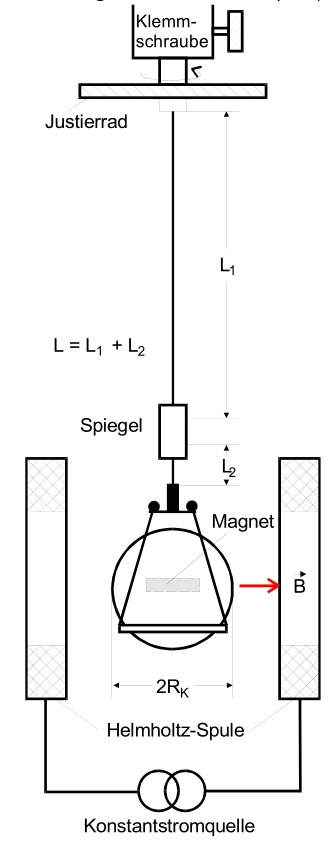
\includegraphics[height=0.5\textwidth]{bilder/aufbau2.jpg}
  \caption{Aufbau zur Bestimmung des magnetischen Moments \cite{102}}
  \label{mess2}
\end{figure}
Der Magnet wird dabei parallel zu den Feldlinien ausgerichtet. Der Strom I, der
an dem Helmholtzspulen-Paar anliegt wird schrittweise erhöht. Die
Schwingungsdauer T wird erneut gemessen.
Abschließend werden die Spulen ausgeschaltet und der Magnet in Nord-Süd-Richtung
ausgerichtet. Die Schwingungsdauer wird gemessen, nachdem das System in
Torsionsschwingung versetzt wurde.
